\section{Casos de Estudo}
\label{sec:chap03_marketstudy}
A investigação neste campo de estudo tem vindo a desenvolver-se desde o século XX~\parencite{survey_nlidb}. Assim sendo, é importante apresentar e examinar os casos mais pertinentes para o protótipo em desenvolvimento neste trabalho, na perspetiva de perceber quais as inovações que cada um deles trouxe para a área das \glspl{ilnbd} e em que medida se enquadram com o problema em resolução.

\subsection{LUNAR}
O LUNAR é um sistema que dá resposta ao domínio de amostras de rochas trazidas da lua e foi o primeiro sistema \gls{ilnbd}~\parencite{nlidb_brief_review, survey_nlidb}. O desenvolvimento deste sistema surgiu da necessidade de possibilitar aos cientistas envolvidos no estudo das rochas lunares poderem obter informação para formular e testar as suas hipóteses, de uma forma simples e intuitiva. O LUNAR permitia ao cientista executar diversas ações como fazer questões, computar médias e taxas, criar listas baseadas em critérios de seleção ou comparar medidas de diferentes investigadores, usando informação de duas bases de dados, uma contendo dados de análises químicas e a outra com dados de referências bibliográficas. Apesar de ter sido desenvolvido como protótipo, este sistema apresentou um desempenho satisfatório, sendo que cerca de 78\% dos pedidos foram respondidos com sucesso~\parencite{lunar_sciences_nlis}.

\subsection{LADDER}
O LADDER é um sistema desenhado para consultar informação sobre navios da Marinha Americana, por forma a auxiliar os gestores da Marinha no processo de tomada de decisão~\parencite{nlidb_brief_review, developing_nli_complex_data}. O sistema, que usa gramática semântica para tratar \textit{queries} a uma base de dados distribuída, apresenta uma arquitetura de três camadas, cada uma correspondente a um componente do sistema: o INLAND -- \textit{Infomal Natural Language Access to Navy Data} --, é responsável por aceitar a \textit{query} de linguagem natural, produzir a respetiva \textit{query} de base de dados a partir da decomposição da mesma em fragmentos, sendo posteriormente combinados para unidades sintáticas a alto nível, para que sejam reconhecidas, dando origem a um comando enviado para o próximo componente; o IDA -- \textit{Intelligent Data Access} --, compõe uma resposta com base no comando recebido e organiza a sequência correta de \textit{queries} a realizar; o FAM -- \textit{File Access Manager} --, o último componente, tem a responsabilidade de gerir o acesso à base de dados distribuída~\parencite{developing_nli_complex_data}.

\subsection{CHAT-80}
Segundo \textcite{nlidb_brief_review}, o CHAT-80 é um dos sistemas \gls{pln} mais referenciados nos anos 80. O CHAT-80 foi desenvolvido pensando na adaptabilidade a diversos domínios, de forma fácil e eficiente. Foi implementado em \textit{Prolog} e incluía uma base de conhecimento com factos geográficos de mais de 150 países (domínio de geografia mundial) e vocabulário inglês suficiente para interação com uma base de dados, que neste caso específico seria implementada totalmente em \textit{Prolog}. Os autores concordaram que a aplicação devia lidar com um conjunto restrito de linguagem natural relevante para o domínio, uma vez que dessa forma se torna uma linguagem de \textit{query} formal mas acessível para o utilizador~\parencite{efficient_easily_adaptable_system_interpreting_nlq}.

\subsection{JANUS}
O JANUS é uma aplicação \gls{pln} com a capacidade de \inquotes{comunicar} com múltiplos sistemas, tais como bases de dados, sistemas periciais, dispositivos gráficos, sendo capaz de avaliar a \textit{query} de linguagem natural e inferir acerca de quais os recursos a utilizar, sem que o utilizador se apercebesse da complexidade do sistema~\parencite{nlidb_brief_review, access_multiple_underlying_system_janus}. O fluxo do JANUS consistia em extrair as expressões da \textit{query} de linguagem natural, usando uma linguagem desenvolvida para o efeito, denominada \textit{World Model Language}; traduzir essas expressões para uma representação simplificada e normalizada; aplicar o algoritmo desenvolvido para encontrar a combinação adequada de serviços a disponibilizar, de modo a satisfazer o pedido do utilizador; por fim, a criação e execução de um plano para extração da informação~\parencite{access_multiple_underlying_system_janus}.

\subsection{PRECISE}
O PRECISE é um sistema desenvolvido na Universidade de Washington, cuja base de dados alvo é relacional, usando \gls{sql}, e que introduz o conceito de frases semanticamente tratáveis, ou seja, \textit{queries} que podem ser traduzidas para uma representação semântica única~\parencite{overview_nlidb_approaches_implementation_airline, nlidb_brief_review}. \textcite{modern_nlidb_composing_statistical_parsing_semantic_tractability} menciona que a distinção entre questões semanticamente tratáveis e as complexas resulta num processo de tratamento da linguagem natural mais simples e pode ser usado para compensar erros de \textit{parsing} sintáticos. 

A Figura~\ref{fig:precise_architecture} apresenta a arquitetura deste sistema, no qual se destaca o \textit{Parser Plugin}, um componente que permite ao PRECISE adaptar-se aos avanços na tecnologia de \textit{parsing}, sem que haja a necessidade de adaptar todo o sistema~\parencite{modern_nlidb_composing_statistical_parsing_semantic_tractability}. 

\begin{figure}[!ht]
    \centering
    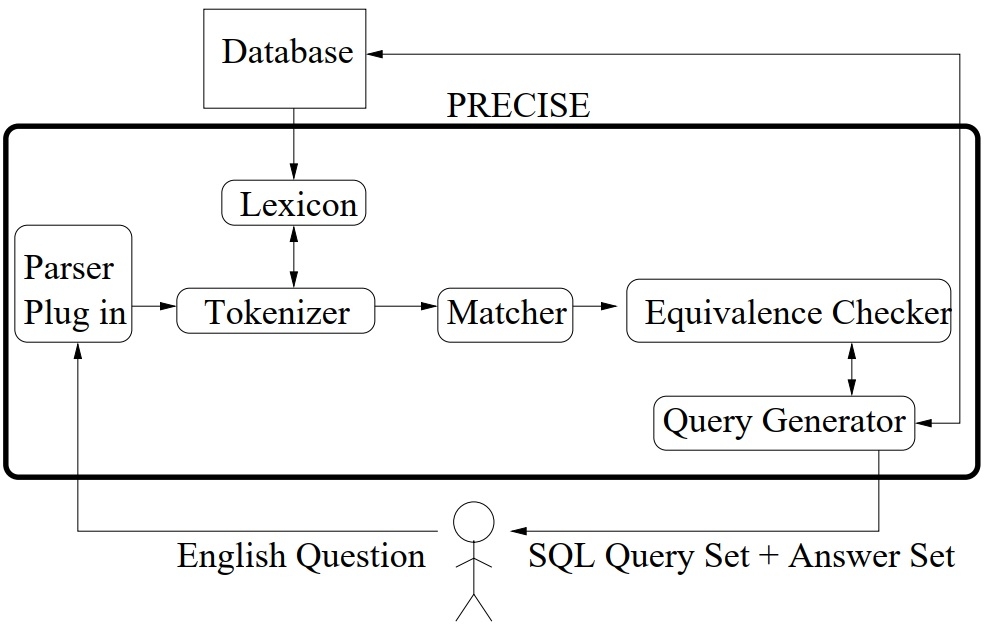
\includegraphics[width=.6\textwidth]{ch03/assets/precise_architecture.jpg}
    \caption{Arquitetura do sistema PRECISE, extraído de~\textcite{towards_theory_nli_databases}}
    \label{fig:precise_architecture}
\end{figure}

Quanto aos restantes componentes: o \textit{Lexicon} extrai os \textit{tokens} de uma dada frase e encontra sinónimos dessas expressões; o \textit{Tokenizer} verifica se, para cada potencial \textit{token}, outras palavras estão também presentes na questão, e associa-lhes um um determinado tipo de elemento de base de dados (\exempligratia{valor, atributo, relação}); o \textit{Matcher} procede à correspondência entre os \textit{tokens} e os respetivos elementos da base de dados; o \textit{Query Generator}, como o próprio nome indica, é responsável por gerar a \textit{query} de \gls{sql}; o \textit{Equivalence Checker} testa se existem soluções distintas e, em caso de as encontrar, o sistema questiona o utilizador acerca da interpretação semântica da questão~\parencite{towards_theory_nli_databases}.

Este sistema foi avaliado em dois domínios: o primeiro, referente a viagens aéreas e o segundo, associado à geografia dos Estados Unidos da América. De acordo com \textcite{nlidb_brief_review}, no primeiro caso, $95.8\%$ das questões são semanticamente tratáveis, pelo que a precisão do sistema atinge os $94\%$ e, no segundo caso, $77.5\%$ das questões são tratáveis em termos de semântica, obtendo $100\%$ de precisão, destacando-se assim o seu desempenho.

\subsection{NALIX}
O NALIX -- \textit{Natural Language Interface for an XML Database} -- é uma \gls{ilnbd} desenvolvida na Universidade de Michigan, com o intuito de obter informação genérica a partir de uma base de dados em \gls{xml}~\parencite{nalix_interactive_nli_querying_xml}. De acordo com~\textcite{nalix_interactive_nli_querying_xml}, o desafio consiste em traduzir uma \textit{query} de linguagem natural para uma \textit{query} corretamente estruturada para uso numa base de dados, permitindo assim ao utilizador usar operações complexas (\exempligratia{agregação, combinação, junção, entre outras}).

Relativamente à arquitetura do NALIX (Figura~\ref{fig:nalix_architecture}), o sistema consiste em duas partes: a primeira é responsável pela tradução da \textit{query} de linguagem natural para XQuery\footnote{Disponível em \url{https://www.w3schools.com/xml/xquery_intro.asp}.}, envolvendo os componentes \textit{Parse Tree Classifier}, \textit{Parse Tree Validator} e \textit{Parse Tree Translator}; a segunda suporta a formulação da \textit{query} de base de dados correspondente, usando os componentes \textit{Query Repository} e \textit{Message Generator}~\parencite{nalix_interactive_nli_querying_xml}.

\begin{figure}[!ht]
    \centering
    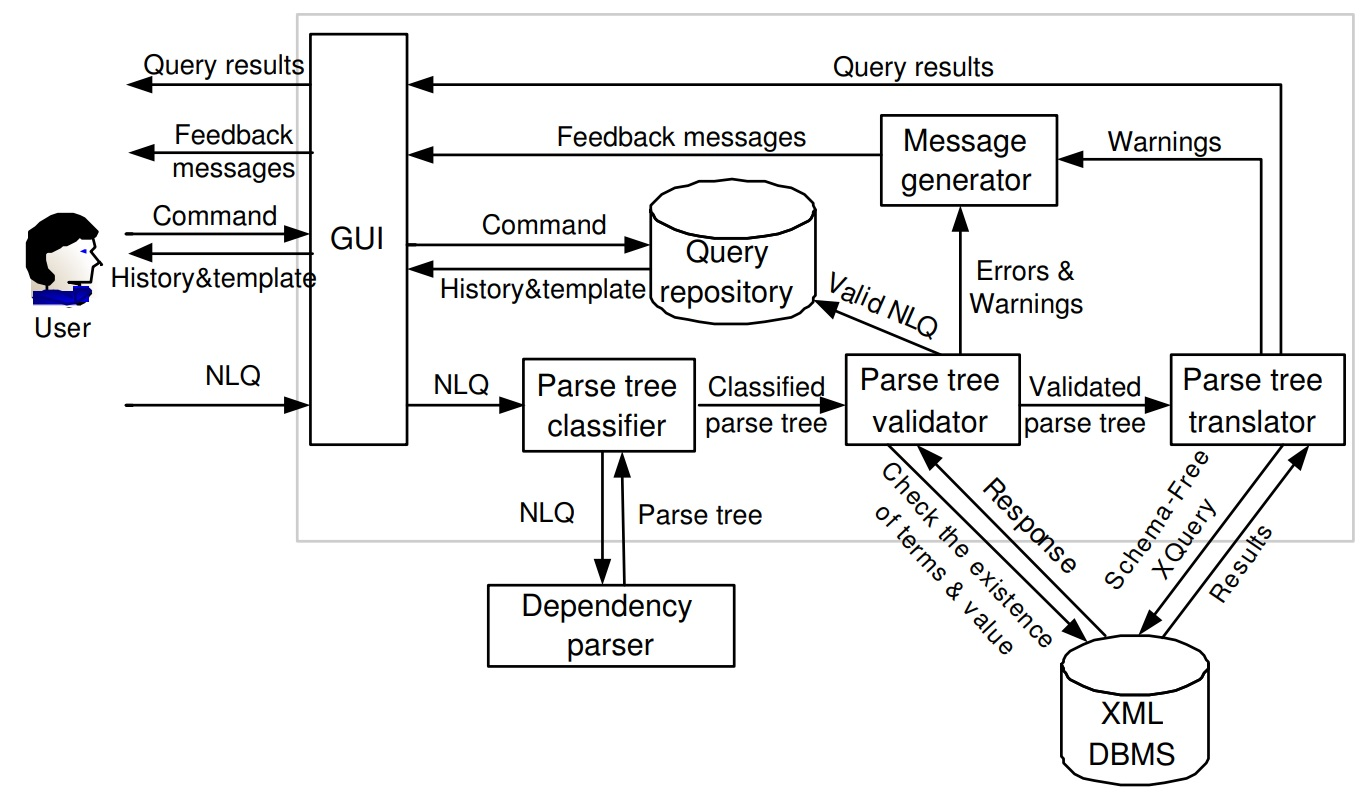
\includegraphics[width=.74\textwidth]{ch03/assets/nalix_architecture.jpg}
    \caption{Arquitetura do sistema NALIX, extraído de~\textcite{nalix_interactive_nli_querying_xml}}
    \label{fig:nalix_architecture}
\end{figure}

De salientar é que a linguagem de \textit{query} usada pelo NALIX (\textit{Schema Free XQuery}) não necessita que seja explicitado qual o \textit{schema} a ser usado, sendo que é capaz de encontrar automaticamente, para uma dada coleção de expressões/palavras-chave, todas as relações existentes entre estes elementos. Assim, é possível abstrair o sistema do domínio existente~\parencite{nalix_interactive_nli_querying_xml, survey_nlidb}.

\subsection{GINLIDB}
Este sistema -- \textit{Generic Interactive Natural Language Interface to Databases} -- foi desenvolvido em 2009 com o propósito de ser genérico o suficiente para se adaptar a bases de dados diferentes, dada a base de conhecimento apropriada~\parencite{ginlidb}. A arquitetura do GINLIDB, apresentada na Figura~\ref{fig:ginlidb_architecture}, consiste em dois principais componentes: \textit{Linguistic Handling Component}, o qual gere a exatidão da \textit{query} de linguagem natural, nomeadamente a estrutura gramatical e possibilidade de ser corretamente convertida para \gls{sql}; \textit{SQL Construting Component}, responsável por construir a \textit{query} de \gls{sql} apropriada e gerir a ligação à base de dados~\parencite{ginlidb}.

\begin{figure}[!ht]
    \centering
    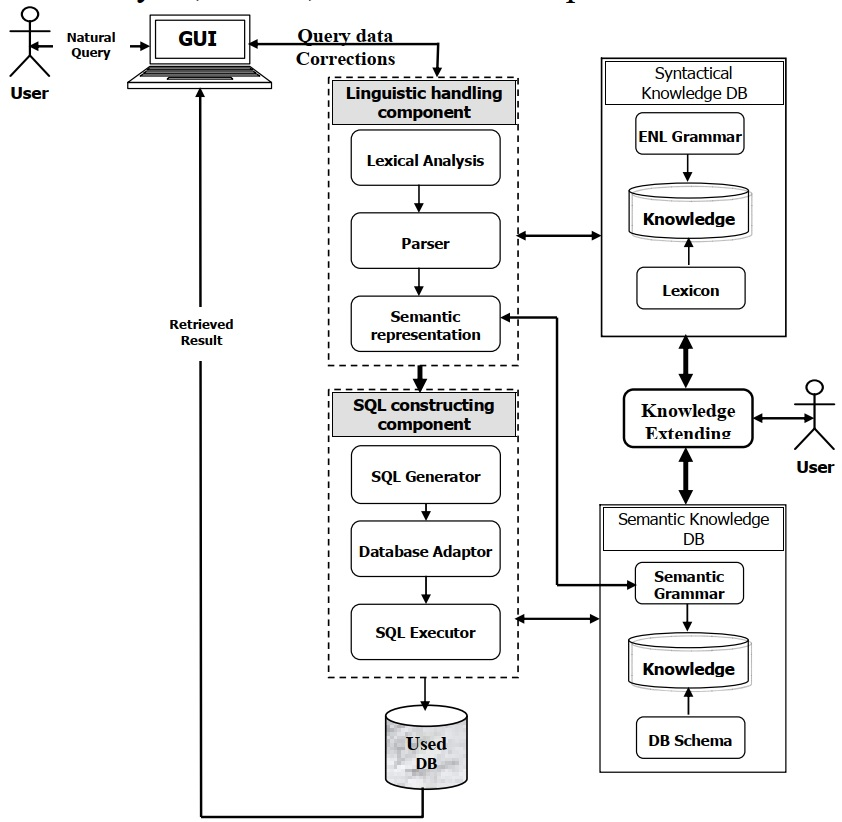
\includegraphics[width=.6\textwidth]{ch03/assets/ginlidb_architecture.jpg}
    \caption{Arquitetura do sistema GINLIDB, extraído de~\textcite{ginlidb}}
    \label{fig:ginlidb_architecture}
\end{figure}

O GINLIDB destaca-se pelo seu processo de análise sintática, no qual usa \gls{atn}, que verifica se a estrutura dos \textit{tokens} é permitida na estrutura gramatical. Este processo é suportado pelo \textit{parser} desenvolvido para o sistema usando uma gramática de contexto livre. Outro destaque deste sistema diz respeito à base de conhecimento usada, que é extensível pelo utilizador, permitindo adicionar novas palavras no dicionário, associar-lhes os respetivos sinónimos e definir o \textit{schema} da base de dados em uso, mapeando assim o domínio. Em termos de resultados, o sistema mostrou-se capaz de responder às questões mais comuns, embora não tenha sido testado em diferentes domínios~\parencite{ginlidb}.

\subsection{Sumário do Casos de Estudo}

\begin{table}[!ht]
\caption{Sumário dos casos de estudo de \gls{ilnbd}}
\label{tab:study_cases}
\centering
\resizebox{\textwidth}{!}{\begin{tabular}{l|l|l|l|l}
%
\toprule
%
\tabhead{Ano}&\tabhead{Nome}&\tabhead{Domínio}&\tabhead{Abordagem}&\tabhead{Técnica}\\ 
%
\midrule
1973 &   LUNAR &   Amostras de rochas da Lua &   bla &   bla\\
1978 &   LADDER &   Navios da Marinha Americana  &   bla &   bla\\
1980 &   CHAT-80 &   Genérico &   bla &   bla\\
1989 &   JANUS &   Genérico &   bla &   bla\\
2004 &   PRECISE &   Viagens aéreas e geografia &   bla &   bla\\
2006 &   NALIX &   Genérico &   bla &   bla\\
2009 &   GINLIDB &   Genérico &   bla &   bla\\
%
\bottomrule
\end{tabular}}
\end{table}